
\documentclass[a4paper,oneside,12pt]{article}

\usepackage[slovene]{babel}    % slovenian language and hyphenation
\usepackage[utf8]{inputenc}    % make čšž work on input
\usepackage[T1]{fontenc}       % make čšž work on output
\usepackage[reqno]{amsmath}    % basic ams math environments and symbols
\usepackage{amssymb,amsthm}    % ams symbols and theorems
\usepackage{url}               % \url and \href for links
\usepackage{icomma}            % make comma a thousands separator with correct spacing
\usepackage{graphicx}          % slike
\usepackage{enumitem}          % seznami
\usepackage[bookmarks, colorlinks=true, linkcolor=black, anchorcolor=black,
  citecolor=black, filecolor=black, menucolor=black, runcolor=black,
  urlcolor=black, pdfencoding=unicode]{hyperref}  % clickable references, pdf toc
\usepackage[
  paper=a4paper,
  top=2.5cm,
  bottom=2.5cm,
  left=2.5cm,
  right=2.5cm
% textheight=24cm,
% textwidtht=16cm,
]{geometry}  % page geomerty

\pagestyle{empty}              % vse strani prazne
\setlength{\parindent}{0pt}    % zamik vsakega odstavka
\setlength{\parskip}{10pt}     % prazen prostor po odstavku
\setlength{\overfullrule}{30pt}  % oznaci predlogo vrstico z veliko črnine

\newenvironment{enumerate*}{\vspace{-1\parskip}\begin{enumerate}\setlength{\itemsep}{0pt}\setlength{\parskip}{2pt}}{\end{enumerate}\vspace{-1\parskip}}
\newenvironment{itemize*}{\vspace{-1\parskip}\begin{itemize}\setlength{\itemsep}{0pt}\setlength{\parskip}{2pt}}{\end{itemize}\vspace{-2.3\parskip}}

\begin{document}

\begin{minipage}[t]{0.7\linewidth}
Študentski svet Fakultete za matematiko in fiziko \\
Jadranska 19 \\
1000 Ljubljana \\

Ljubljana, \today\\
\end{minipage}%
\begin{minipage}[t]{0.3\linewidth}
  \mbox{} \\[-15pt]
  \hspace*{\fill} 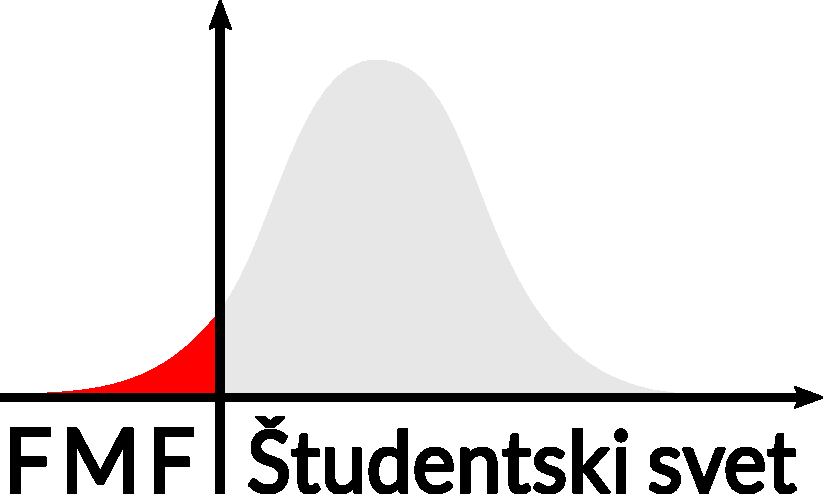
\includegraphics[width=0.9\linewidth]{ssfmf_logo_col.pdf}
\end{minipage}

Fakulteta za matematiko in fiziko \\
Jadranska 19 \\
1000 Ljubljana \\

\textbf{ZADEVA: Rezultati volitev v ŠS FMF 2018/19}

Volilna komisija v sestavi Žiga Avbreht, Matej Jazbec in Luka Miklavčič je po koncu glasovanja preštela oddane
glasove. Oddanih je bilo 96 veljavnih in 1 neveljavna
glasovnica. Rezultati so predstavljeni v tabeli~\ref{tab:rez}.

\begin{table}[!h]
    \centering
    \begin{tabular}{|l|r|} \hline
\textbf{Ime	in priimek} & \textbf{Št.\ glasov} \\ \hline
Klementina Pirc & 41 \\ \hline
Jure Slak & 41 \\ \hline
Matej Janežič & 39\\ \hline
Ines Meršak & 39 \\ \hline
Rok Kaufman & 34 \\ \hline
Aljoša Rebolj & 34 \\ \hline
Miha Srdinšek & 34 \\ \hline
Pia Klemenc & 33 \\ \hline
Katarina Šipec & 32 \\ \hline
    \end{tabular}
    \caption{Število glasov, ki so jih prejeli kandidati.}
    \label{tab:rez}
\end{table}

Volilna komisija ugotavlja, da so vsi kandidati izvoljeni v ŠS FMF.

\vspace{5ex}

\hspace*{\fill} Matej Jazbec \\
\hspace*{\fill} Predsednik volilne komisije

\end{document}
